\documentclass[a4paper, 11pt]{article}
\usepackage{amsmath}
\usepackage[utf8]{inputenc}
\usepackage[spanish]{babel}
\usepackage{wrapfig, framed, caption}
\usepackage[usenames, dvipsnames]{color}
\usepackage{amssymb}
\usepackage[a4paper, total={7in, 9in}]{geometry}
\usepackage{graphicx}
\usepackage{float}
\usepackage{subcaption}
\usepackage{multicol}
\usepackage{xcolor}
\usepackage{hyperref}
\usepackage{verbatim}
\usepackage{enumitem}

%de proba
\def\P{{\mathbf P}}
\def\E{{\mathbf E}}
\def\cov{{\bf cov}}
\def\var{{\bf var}}

\begin{document}

\begin{center}
\centerline{\bf Estadística 1 (Química)}%
\vspace{0.2cm}


\textbf{Práctica 4 - Estadística Descriptiva\vspace{-0.1in}}
\end{center}


\begin{enumerate}
\item Una muestra estándar de suero sanguíneo contiene $42.0$ g de
albúmina por litro. Cuatro laboratorios (A -- D) realizan seis
determinaciones cada uno (en el mismo día) de la concentración de
albúmina, con los siguientes resultados (en g/l):%
\[%
\begin{tabular}
[c]{|c|}\hline
A\qquad42.5\qquad41.6\qquad42.1\qquad41.9\qquad41.1\qquad42.2\\
B\qquad39.8\qquad43.6\qquad42.1\qquad40.1\qquad43.9\qquad41.9\\
C\qquad43.5\qquad42.8\qquad43.8\qquad43.1\qquad42.7\qquad43.3\\
D\qquad39.4\qquad41.9\qquad40.7\qquad40.3\qquad42.6\qquad39.0\\\hline
\end{tabular}
\ \
\]
(para resolver este ejercicio, mire las instrucciones en el archivo
\texttt{instruccionesej1.R} cuyo link figura cerquita de dónde bajó
este archivo).


\begin{enumerate}
\item Grafique en cada caso los datos en un Diagrama de Punto, todos en la
misma escala.


\item Comente la exactitud y la precisión de los resultados de las mediciones de cada uno de los laboratorios. ¿Qué variables aleatorias puede utilizar para aproximar el grado de dispersión y la exactitud de las muestras?
\end{enumerate}


\item En un experimento se midió la temperatura de fusión del
indio y del azufre. Los datos figuran más adelante. La siguiente
instrucción puede ser útil para leer el archivo en R (ya que las
longitudes de los dos conjuntos de datos son diferentes).%
\[
\text{\texttt{read.table(file.choose(),head=TRUE,fill=TRUE)}}%
\]

\begin{enumerate}
\item \label{2a} Compare los dos conjuntos de datos mediante histogramas y boxplots.
Realice un gráfico de boxplots paralelos.


\item Halle las medias, las medianas y las medias podadas al 10\% y 20\%. Compare.


\item Halle el desvío estándar, la distancia intercuartil y la MAD
como medidas de dispersión.


\item \label{2d} Halle los percentiles muestrales 0.90, 0.75, 0.50, 0.25 y 0.10.


\item Las temperaturas se toman en orden cronológico y se considera que se ha llegado al punto de fusión cuando la temperatura se estabiliza ¿Es razonable
el modelo de errores independientes e idénticamente distribuidos?
¿Sería correcto analizar todo el conjunto de datos?
¿A partir de cuál observación considera que el
proceso se ha estabilizado?


\item Sobre el conjunto de datos correspondiente al proceso estabilizado, resuelva nuevamente los ítems \ref{2a}) al \ref{2d}).%

\[%
\begin{tabular}
[c]{|c|}\hline
INDIO \\\hline
136.6\qquad145.2\qquad151.5\qquad162.7\qquad159.1\qquad159.8\qquad
160.8\qquad173.9\qquad160.1\\
160.4\qquad161.1\qquad160.6\qquad160.2\qquad159.5\qquad160.3\qquad
159.2\qquad159.3\qquad159.6\\
160.0\qquad160.2\qquad160.1\qquad160.0\qquad159.7\qquad159.5\qquad
159.5\qquad159.6\qquad159.5\\\hline
\end{tabular}
\ \
\]%
\[%
\begin{tabular}
[c]{|c|}\hline
AZUFRE \\\hline
126.4\qquad135.7\qquad132.9\qquad131.5\qquad131.1\qquad131.1\qquad
131.9\qquad132.7\\
133.3\qquad132.5\qquad133.0\qquad133.0\qquad132.4\qquad131.6\qquad
132.6\qquad132.2\\
131.3\qquad131.2\qquad132.1\qquad131.1\qquad131.4\qquad131.2\qquad
131.1\qquad131.1\\\hline
\end{tabular}
\ \
\]


\end{enumerate}


\item En un estudio nutricional se consideran las calorías y el
contenido de sodio de tres tipos de salchichas y se obtuvieron los datos que
se muestran en la tabla final.


\begin{enumerate}
\item \label{3a} Realice un histograma para las calorías de cada tipo de salchichas.
\textquestiondown Observa grupos en algún gráfico?
\textquestiondown Cuántos grupos observa? \textquestiondown Observa
algún candidato a outlier?


\item Repita el ítem anterior para la cantidad de sodio.


\item Realice un gráfico de boxplots paralelos de las calorías versus tipo de salchichas.
¿Observa alguna relación entre cada uno de de los boxplots y los histogramas realizados en el item \ref{3a})? A qué conclusión llega? De acuerdo con los boxplots
hallados, \textquestiondown cómo caracterizaría la diferencia entre los tres tipos de salchichas desde el punto de vista de las calorías?%

\[%
\begin{tabular}
[c]{|c|c|c|c|c|c|}\hline
\multicolumn{2}{|c|}{A} & \multicolumn{2}{|c|}{B} & \multicolumn{2}{|c|}{C}%
\\\hline
Calorías & Sodio & Calorías & Sodio & Calorías & Sodio\\\hline
186 & 495 & 173 & 458 & 129 & 430\\
181 & 477 & 191 & 506 & 132 & 375\\
176 & 425 & 182 & 473 & 102 & 396\\
149 & 322 & 190 & 545 & 106 & 383\\
184 & 482 & 172 & 496 & 94 & 387\\
190 & 587 & 147 & 360 & 102 & 442\\
158 & 370 & 146 & 387 & 87 & 359\\
139 & 322 & 139 & 386 & 99 & 357\\
175 & 479 & 175 & 507 & 170 & 528\\
148 & 375 & 136 & 393 & 113 & 513\\
152 & 330 & 179 & 405 & 135 & 426\\
111 & 300 & 153 & 372 & 142 & 513\\
141 & 386 & 107 & 144 & 86 & 358\\
153 & 401 & 195 & 511 & 143 & 581\\
190 & 645 & 135 & 405 & 152 & 588\\
157 & 440 & 140 & 428 & 146 & 522\\
131 & 317 & 138 & 339 & 144 & 545\\
149 & 319 &  &  &  & \\
135 & 298 &  &  &  & \\
132 & 253 &  &  &  & \\\hline
\end{tabular}
\ \
\]


\end{enumerate}


\item[4.] Los siguientes datos corresponden a 100 determinaciones repetidas de
la concentración de ion nitrato (en $\mu$mol/L). 50 de estas determinaciónes corresponden a
un grupo de estudiantes (Grupo A) y las restantes 50 a otro grupo (Grupo B):%
\[%
\begin{tabular}
[c]{|cccc|cccc|}\hline
\multicolumn{4}{|c|}{Grupo A} & \multicolumn{4}{|c|}{Grupo B}\\\hline
0.51 & 0.51 & 0.50 & 0.50 & 0.61 & 0.67 & 0.70 & 0.56\\
0.51 & 0.50 & 0.48 & 0.50 & 0.61 & 0.67 & 0.63 & 0.75\\
0.49 & 0.50 & 0.47 & 0.50 & 0.55 & 0.49 & 0.75 & 0.55\\
0.51 & 0.48 & 0.52 & 0.49 & 0.65 & 0.77 & 0.64 & 0.58\\
0.51 & 0.49 & 0.52 & 0.51 & 0.73 & 0.51 & 0.66 & 0.65\\
0.51 & 0.48 & 0.52 & 0.49 & 0.65 & 0.57 & 0.61 & 0.53\\
0.52 & 0.53 & 0.49 & 0.51 & 0.53 & 0.64 & 0.52 & 0.69\\
0.48 & 0.51 & 0.50 & 0.47 & 0.54 & 0.57 & 0.63 & 0.62\\
0.51 & 0.49 & 0.50 & 0.50 & 0.68 & 0.56 & 0.58 & 0.58\\
0.50 & 0.49 & 0.53 & 0.47 & 0.59 & 0.62 & 0.60 & 0.66\\
0.51 & 0.50 & 0.49 & 0.48 & 0.61 & 0.54 & 0.63 & 0.61\\
0.53 & 0.52 & 0.51 & 0.51 & 0.69 & 0.63 & 0.53 & 0.48\\
0.46 & 0.49 &  &  & 0.65 & 0.61 &  & \\\hline
\end{tabular}
\
\]




\begin{enumerate}
\item Estudie si la distribución de los conjuntos de datos para ambos
grupos es normal, realizando los correspondientes histogramas y superponiendo
la curva normal. ¿Llega a la misma conclusión realizando qqplots para cada conjunto de datos?


\item \textquestiondown A partir de los valores observados, le parece razonable asumir que ambos grupos están midiendo el mismo mesurando? Responda comparando medidas de centralidad y de
dispersión de los datos. Hacer un gráfico de boxplots paralelos que permita comparar las distribuciones de ambos conjuntos de datos.
\end{enumerate}


\item[5.] En una clase grande, hay 150 estudiantes hombres y 100 mujeres, los
estudiantes promediaban en altura 178cm, con un desvío standard de 25cm y
las estudiantes promediaban 162cm, con un desvío standard de 25cm.
Tomando conjuntamente los hombres y las mujeres:


\begin{enumerate}
\item Determine la altura promedio.

\item Indique si el desvío estándar de las alturas es
mayor que 25cm, exactamente 25cm, ó inferior a 25cm.
\end{enumerate}


\item[6.] Con la finalidad de determinar el contenido de Arsénico Ar2+ en ríos de la patagonia, se midió potenciométricamente la concentración en ppb del ión Ar2+ de dos ríos a distintas alturas de su desembocadura. Sea $x_1, \ldots, x_n$ las mediciones realizadas para el primer río y $y_1, \ldots, y_n$ las mediciones del segundo río. Se sabe que la altura en que se midió el contenido de arsénico de $x_i$ es el mismo que $y_i$, para $1 \leq i \leq 26$.

Las siguientes tablas presentan la cantidad de arsénico en ppb medido en ambos ríos.%
\[%
\begin{tabular}
[c]{|c|}\hline
CONTENIDO DE AR2+ RIO A\\\hline
129.6\qquad31.4\qquad2745.6\qquad489.1\qquad430.0\qquad302.8\qquad
119.0\qquad4.1\qquad92.4\\
17.5\qquad200.7\qquad274.7\qquad274.7\qquad7.7\qquad1656.0\qquad
978.0\qquad198.6\qquad703.4\\
1697.8\qquad334.1\qquad118.3\qquad255.0\qquad115.3\qquad242.5\qquad
32.7\qquad40.6\\\hline
\end{tabular}
\
\]%
\[%
\begin{tabular}
[c]{|c|}\hline
CONTENIDO DE AR2+ RIO B\\\hline
26.1\qquad26.3\qquad87.0\qquad95.0\qquad372.4\qquad0.01\qquad17.3\qquad
24.4\qquad11.5\\
321.2\qquad68.5\qquad81.5\qquad47.3\qquad28.6\qquad830.1\qquad345.5\qquad
1202.6\qquad36.6\\
4.9\qquad4.9\qquad41.1\qquad29.9\qquad163.0\qquad244.3\qquad147.8\qquad
21.7\\\hline
\end{tabular}
\
\]




\begin{enumerate}
\item Realice boxplots para ambos grupos. ¿Le parece que el
contenido medio de arsénico de los ríos difiere?


\item Analice la normalidad realizando\ qqplots e histogramas (de densidad) para ambos conjuntos de datos y superponiendo la curva normal.

\item Realice la transformación log a los datos y repita el item anterior para los datos transformados.

\end{enumerate}


\item El histograma muestra la distribución de presión
sanguínea de 15000 mujeres en estudio. Utilice el histograma para
responder las siguientes preguntas:%


%TCIMACRO{\FRAME{fhF}{3.3261in}{2.5521in}{0pt}{}{}{histogramadescriptiva.jpg}%
%{\special{ language "Scientific Word";  type "GRAPHIC";
%maintain-aspect-ratio TRUE;  display "USEDEF";  valid_file "F";
%width 3.3261in;  height 2.5521in;  depth 0pt;  original-width 3.2811in;
%original-height 2.5105in;  cropleft "0";  croptop "1";  cropright "1";
%cropbottom "0";
%filename 'histogramadescriptiva.JPG';file-properties "XNPEU";}}}%
%BeginExpansion
\begin{figure}
[ht]
\begin{center}
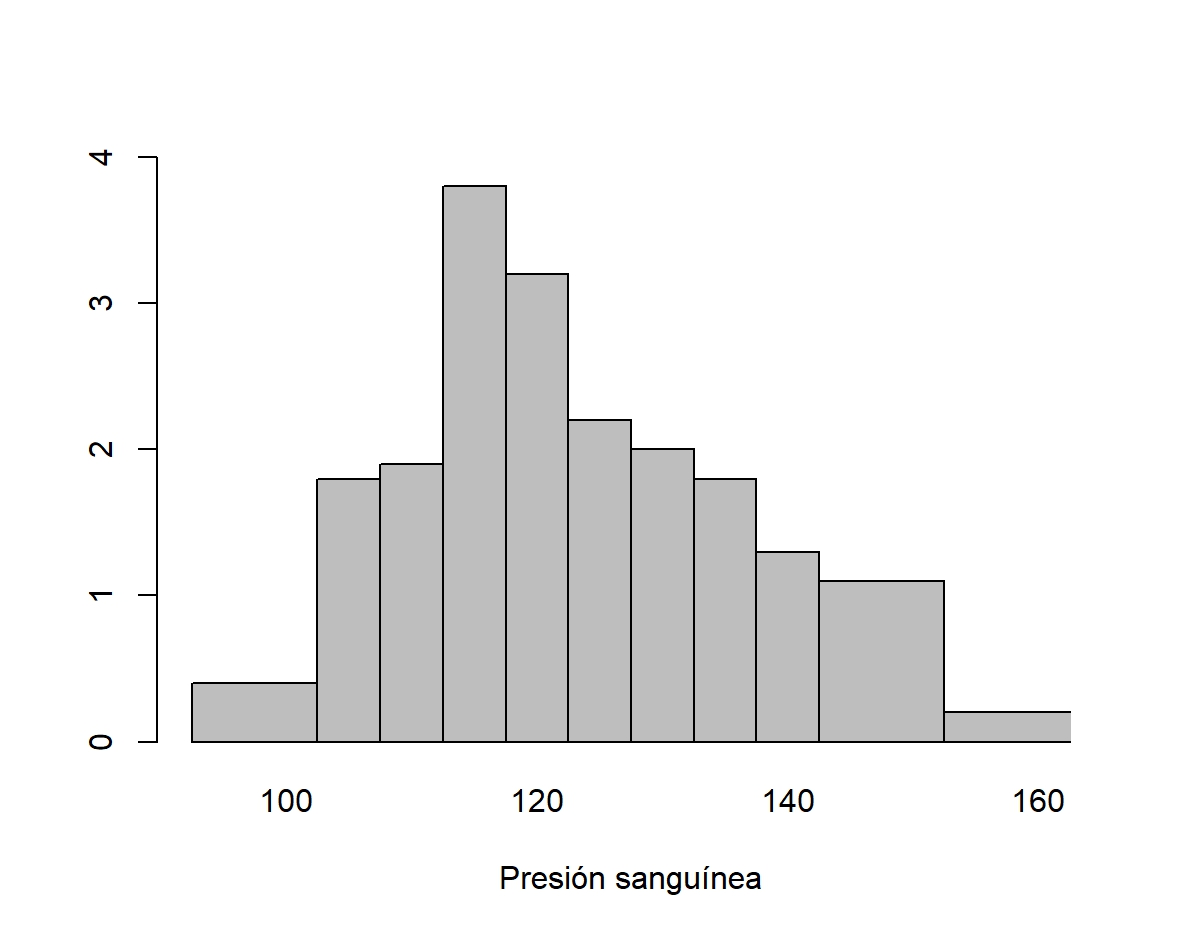
\includegraphics[width=0.75\textwidth]
{imagenes/histogramadescriptiva2025.jpeg}%
\end{center}
\end{figure}
%EndExpansion




\begin{enumerate}
\item \textquestiondown El porcentaje de mujeres con presión superior a
los 130mm es más cercano a 25\%, 50\% o 75\%?


\item \textquestiondown El porcentaje de mujeres con presión entre 90 y
160mm es más cercano al 1\%, 50\% o 99\%?


\item \textquestiondown Cuál intervalo tiene más mujeres: 130-140mm o 140-150mm?


\item \textquestiondown Cuál intervalo tiene más mujeres: 130-135mm o 140-150mm?


\item En el intervalo 125-130mm la altura del histograma es de alrededor de
2.2\% por mm. \textquestiondown Qué porcentaje de mujeres tuvo presión
en ese intervalo?
\end{enumerate}


\item[8.] Considere $x_{1},\ldots,x_{n}$ una muestra de una población
cualquiera. Sean $\overline{x}$ y $\widetilde{x}$\ la media y la mediana
muestral respectivamente.


\begin{enumerate}
\item Si se suma una constante $a$ a cada uno de los $x_{i}$ de la muestra,
obteniéndose $y_{i}=x_{i}+a$, \textquestiondown cómo se relacionan
$\overline{x}$ con $\overline{y}$ y $\widetilde{x}$ con $\widetilde{y}$?


\item Si cada uno de los $x_{i}$ es multiplicado por una constante $b$,
obteniéndose $y_{i}=bx_{i}$, \textquestiondown cómo se relacionan
$\overline{x}$ con $\overline{y}$ y $\widetilde{x}$ con $\widetilde{y}$? ¿Qué sucede si $b$ es positivo o negativo?
\end{enumerate}


\item[9.] Sea $s_{X}^{2}$ la varianza muestral correspondiente a los datos
$x_{1},\ldots,x_{n}$ observados. Demuestre que


\begin{enumerate}
\item $s_{X}^{2}=\frac{1}{n-1}\sum_{i=1}^{n}x_{i}^{2}-\frac{n}{n-1}%
\overline{x}^{2}$.


\item Probar que si $y_{i}=x_{i}+a$ con $a$\ constante, entonces $s_{X}=s_{Y}$.


\item Probar que si $y_{i}=bx_{i}$ con $b$\ constante, entonces $s_{X}%
=\left\vert b\right\vert s_{Y}$.
\end{enumerate}
\end{enumerate}




\end{document}
